\textnormal{
Building the corresponding relational tables, according to the proposed ER model described in the previous phase enforcing the different integrity constraints.  
The deliverables for this stage include the following items (Please refer to the original Project Description for more details):
\begin{itemize} 
\item{}
The SQL tables that represent the ER project model, along with at least 3-5 rows of concrete data per table.
\item{}
The normalization steps for each table, along with explanations/justifications of each normalization step.
\item{}
The SQL table after the normalization steps (showing all table attributes).
\item{}
The SQL statements used to create the SQL tables, including the required triggers as well as the integrity constraints. At least 2 triggers and 2 of each of the following constraint types have to exist in the project tables overall: 
\begin{itemize} 
\item{}
	Data-range constraints for certain fields (for example: the age field should be between 10 and 99, while all other entries should be rejected by the system).
\item{}
	Whether some users will be denied access and/or updates to some data according to their roles (for example: student1 can not access other students' ' grades, so a violation error pops up upon that action. Another example: a sales person can see an item price, but can not change it, since only a manger can, also a violation error pops up upon that update attempt).
\end{itemize}
\item{}
So each table should be followed by the following items:
\begin{itemize} 
\item{}
	Explanation for each constraint, providing examples of certain data access and/or update restrictions per user type. 
\item{}
	Explanation/justification for each trigger, providing examples of certain data access and/or updates per user type. 
\end{itemize}
\end{itemize}
Please insert your deliverables for Stage3 as follows:
\begin{itemize} 
\item{ The SQL Table, including data entries: }
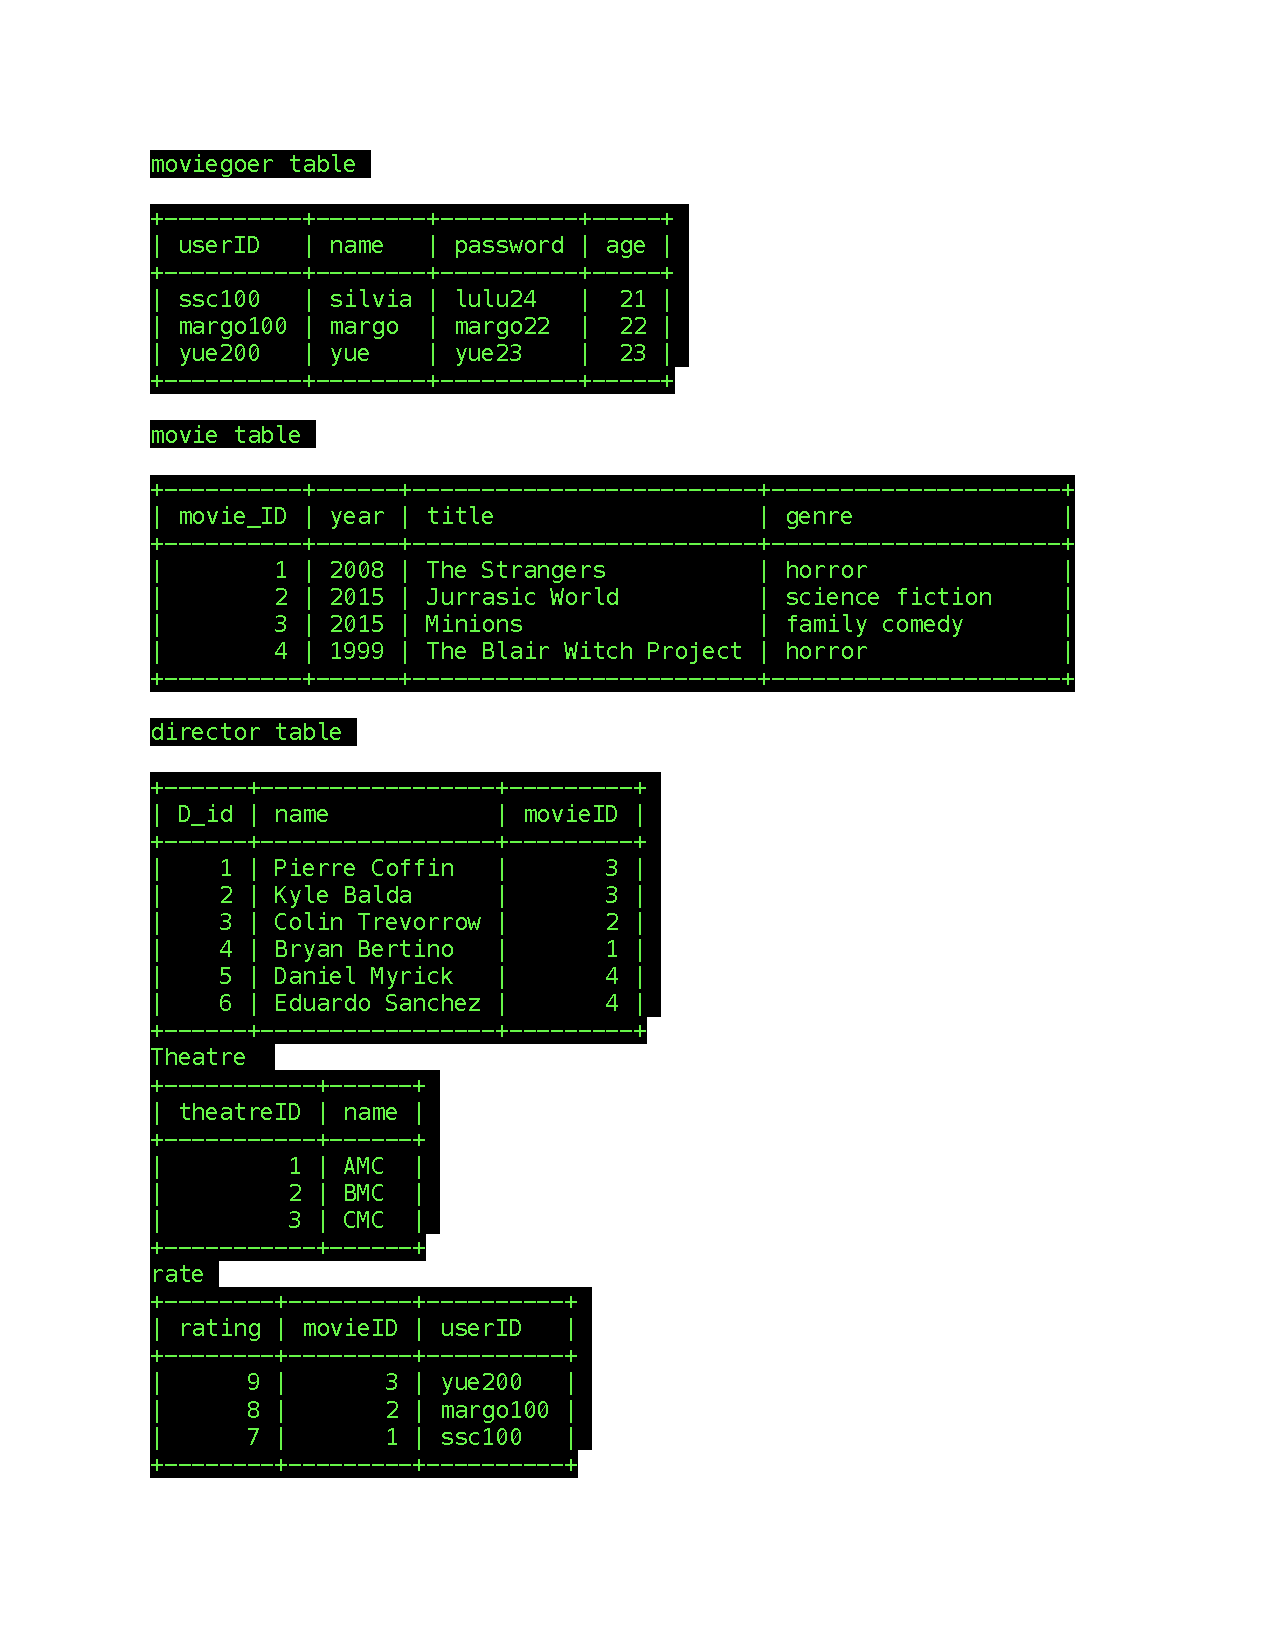
\includepdf[pages={1,2,3}]{tables.pdf}
\item{The normalization steps for each table, along with explanations/justifications: }
The normalization steps should be inserted as follows.
\begin{itemize} 
	\item{The normalization step for the SQL table: }
	Theater Normalization already in 3NF
	\item{The explanations/justification of the normalization step: }
	 It passes 1NF because each attribute can only have one value in a given row. Each theater has one ID and one name.  It passes 2NF and 3NF because the only non-key attribute, name, attribute follows from the theaterID, which is the primary key.
\end{itemize}
\begin{itemize} 
	\item{The normalization step for the SQL table: }
	Showing Normalization already in 3NF
	\item{The explanations/justification of the normalization step: }
	 It passes 1NF because each attribute can only have one value in a given row. Each showing has only one ID, place, date, time, and movie being shown.  It passes 2NF and 3NF because the non-key attributes depend on the entire primary key alone.  The place, date, time, and movie are all independent from each other, and only follow from the showID.
\end{itemize}
\begin{itemize} 
	\item{The normalization step for the SQL table: }
	HasTicket Normalization already in  3NF
	\item{The explanations/justification of the normalization step: }
	 It passes 1NF because each attribute can only have one value in a given row.  Each row consists of only one moviegoer with one amount of tickets for one showing.  It passes 2NF and 3NF because the non-key attribute, number of tickets, depends on the entire primary key alone.  The number of tickets relies on being for a particular moviegoer to use at a particular showing- in other words, both parts of the primary key.
\end{itemize}
\begin{itemize} 
	\item{The normalization step for the SQL table: }
	Rate Normalization already in 3NF
	\item{The explanations/justification of the normalization step: }
	It passes 1NF because each attribute can only have one value in a given row. Each rate consists of 		one rating from one moviegoer for one movie. It passes 2NF and 3NF because the non-key attribute, 	rating, depend on the entire primary key alone.   The rating is from a specific moviegoer for a specific 	movie, so it relies on both parts of the primary key.
\end{itemize}
\begin{itemize} 
	\item{The normalization step for the SQL table: }
	moviegoer Normalization already in 3NF
	\item{The explanations/justification of the normalization step: }
	it passes 1NF because each attribute can only have one value in each row. Each moviegoer has a 		unique userID. it passes 2NF and 3NF because the non key attributes depend on the entire primary 		key alone. super key being movie ID . year, title and genre are all independent from each other 
\end{itemize}
\begin{itemize} 
	\item{The normalization step for the SQL table: }
	movie Normalization already in 3NF
	\item{The explanations/justification of the normalization step: }
	it passes 1NF because each attribute can only have one value in each row. Each movie has a 		unique movie ID. . it passes 2NF and 3NF because the non key attributes depend on the entire primary 		key alone. primary key being user ID . name, password, and age are all independent from each other 
\end{itemize}
\begin{itemize} 
	\item{The normalization step for the SQL table: }
	director Normalization already in 3NF
	\item{The explanations/justification of the normalization step: }
	it passes 1NF because each attribute can only have one value in each row. Each director has a unique director ID.  It passes 2NF and 3NF because the non-key attribute, rating, depend on the entire primary key alone. There can be many directors for a movie so the director is from a specific movie and has a unique Director ID 
\end{itemize}
\begin{itemize} 
	\item{The normalization step for the SQL table: }
	Employee Normalization already in 3NF
	\item{The explanations/justification of the normalization step: }
	It passes 1NF because each attribute can only have one value in a given row. Each employee has one ID one type and one name.� It passes 2NF and 3NF because the non-key attributes, name and type, attribute follows from the EmployeeID, which is the primary key
\end{itemize}
\begin{itemize} 
	\item{The normalization step for the SQL table: }
	employeeWorkin Normalization already in 3NF
	\item{The explanations/justification of the normalization step: }
	It passes 1NF because each attribute can only have one value in a given row. Each hasEmployee has only one theatreID and employeeID being shown.� It passes 2NF and 3NF because there is no non-key attributes in the table. 
\end{itemize}
\begin{itemize} 
	\item{The normalization step for the SQL table: }
	Theatremanagedby Normalization already in 3NF
	\item{The explanations/justification of the normalization step: }
	It passes 1NF because each attribute can only have one value in a given row. Each Theatremanagedby has only one theatreID and theatremanagerID being shown.� It passes 2NF and 3NF because there is no non-key attributes in the table. 
\end{itemize}
\begin{itemize} 
	\item{The normalization step for the SQL table: }
	govern Normalization already in 3NF
	\item{The explanations/justification of the normalization step: }
	It passes 1NF because each attribute can only have one value in a given row.  It passes 2NF and 3NF because there is no non-key attributes in the table. the attributes are all foreign keys 
\end{itemize}
\begin{itemize} 
	\item{The normalization step for the SQL table: }
	supervise Normalization already in 3NF
	\item{The explanations/justification of the normalization step: }
	It passes 1NF because each attribute can only have one value in a given row. It passes 2NF and 3NF because there is no non-key attributes in the table. 
\end{itemize}
\begin{itemize} 
	\item{The normalization step for the SQL table: }
	Showingmanagedby Normalization already in 3NF
	\item{The explanations/justification of the normalization step: }
	 It passes 1NF because each attribute can only have one value in a given row. Each Showingmanagedby has only one showingID and showingmanagerID being shown.� It passes 2NF and 3NF because there is no non-key attributes in the table
\end{itemize}
\begin{itemize} 
	\item{The normalization step for the SQL table: }
	superior Normalization already in 3NF
	\item{The explanations/justification of the normalization step: }
	  It passes 1NF because each attribute can only have one value in a given row. Each superior has only one employeeID and supervisorID being shown.� It passes 2NF and 3NF because the non-key attributes, supervisorID, attribute follows from the employeeID, which is the primary key
\end{itemize}
\item{The SQL statement to create the table: }
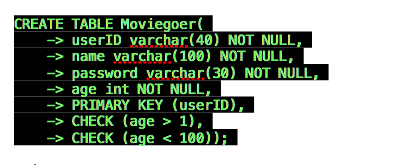
\includegraphics[scale=0.3]{moviegoertable.png}
\item{The Triggers used in the statement: }
Please insert the triggers are as follows:
\begin{itemize} 
	\item{The Trigger: }
	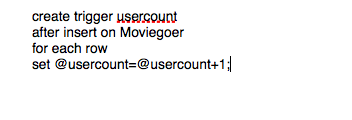
\includegraphics[scale=0.3]{usercount.png}
	\item{The Trigger Explanation/Justification: }
	a count that is added 1 after every insert on the moviegoer table to count how many moviegoers are in the system
	\item{The Trigger Examples (in correlation with the user(s) interaction with the system): }
	the theater manager wants to see how many moviegoers are in his theater ,he can just summon this trigger customer count
\end{itemize}
\item{The Data Range Constraints used in the statement: }
Please insert the Data Range Constraints as follows:
\begin{itemize} 
	\item{The Data Range Constraint: }
	Age in the moviegoer table must be between 1 and 100
	\item{The Data Range Constraint Explanation:}
	ages 1 to 100 are common for a typical person
	\item{The Data Range Constraint Example(s) (in correlation with the user(s) interaction with the system): } 
	A person who is 25, puts their age as 25 and is accepted and valid another example is if the user puts in 255 but the last 5  is put in by mistake, the system will not take age 255 so the insert is invalid
	\item{The Data Access/update Constraint: }
	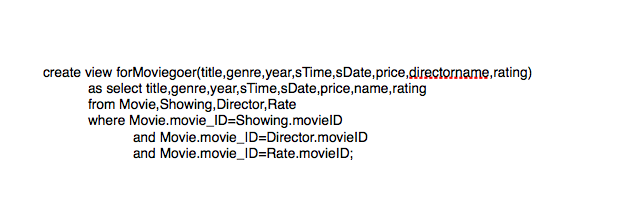
\includegraphics[scale=0.3]{moviegoerview.png}
	\item{The Data Access/update Constraint Explanation:}
	For the moviegoer view , the moviegoer (client) cannot look at other users ID or passwords, name of employees or what type is each employee therefore, we create a view solely for the moviegoer , so they can have access to the movie titles, year, genre, date, time,directors, price and theater name so the moviegoer is able to search movies by director, by title, by date, time and a moviegoer is also able to see price so they can buy tickets 
	\item{The Data Access/update Constraint Example(s) (in correlation with the user(s) interaction with the system): } 
	When a moviegoer goes to buy a ticket  and wants to search by title.They search by title ?the strangers ? and find the times for it and price and go ahead and buy the ticket 
	\item{The Data Access/update Constraint: }
	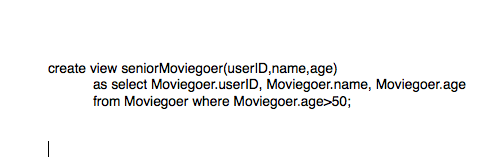
\includegraphics[scale=0.3]{seniormoviegoer.png}
	\item{The Data Access/update Constraint Explanation:}
	The senior moviegoer view is for employees , so they know who is a senior out of their customers , so they can get benefits , such as lower ticket price.
	\item{The Data Access/update Constraint Example(s) (in correlation with the user(s) interaction with the system): } 
	For example if its senior Day , which is when seniors get a free movie ticket to any movie , the theater can give it to them based on this view. This view lists all senior users that exist.  
\end{itemize}
\item{The SQL statement to create the table: }
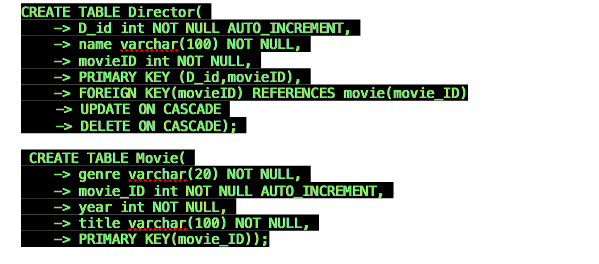
\includegraphics[scale=0.3]{tables1.png}
\item{The Triggers used in the statement: }
Please insert the triggers are as follows:
\begin{itemize} 
	\item{The Trigger: }
	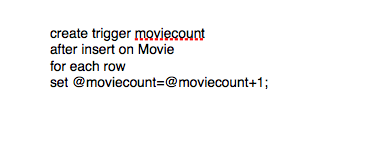
\includegraphics[scale=0.3]{moviecount.png}
	\item{The Trigger Explanation/Justification: }
	a count variable in which one is added every time a movie is added to the system so any of the managers can know how many movies are added to their movie theater system.
	\item{The Trigger Examples (in correlation with the user(s) interaction with the system): }
	a theater manager wants to know how many movies his theater has
\end{itemize}
\item{The SQL statement to create the table: }
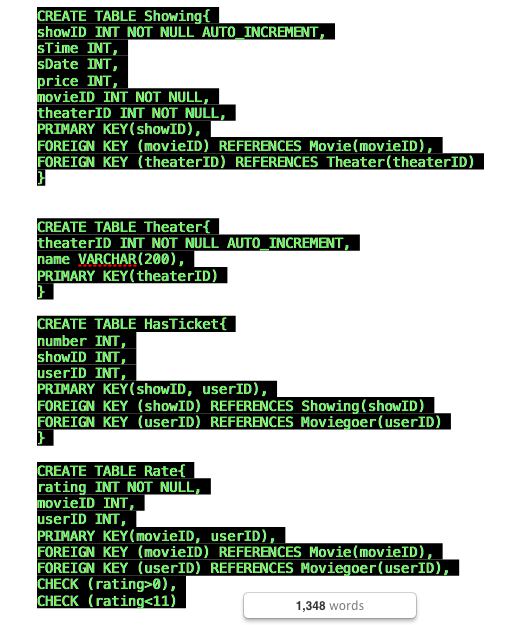
\includegraphics[scale=0.3]{tables2.png}
\item{The Data Range Constraints used in the statement: }
Please insert the Data Range Constraints as follows:
\begin{itemize} 
	\item{The Data Range Constraint: }
	A rating in the 'rate' table must be between one and ten.  
	\item{The Data Range Constraint Explanation:}
	 A ten point scale is a common one for movie ratings, with 10 being the highest possible rating (the movie was fantastic) and one being the lowest (the movie was terrible).  A movie must be rated within the scale for the information to be useful.
	\item{The Data Range Constraint Example(s) (in correlation with the user(s) interaction with the system): } 
	A moviegoer tries to rate a movie they love a 15, but it is rejected because it is off the rating scale.  They then rate the movie 10, and it is accepted.
\end{itemize}
\item{The SQL statement to create the table: }
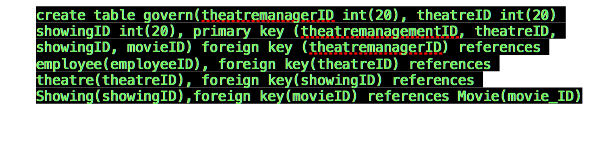
\includegraphics[scale=0.3]{create.png}
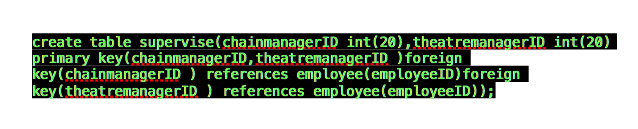
\includegraphics[scale=0.3]{create1.png}
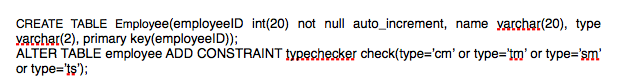
\includegraphics[scale=0.3]{emptables.png}
\item{The Data Range Constraints used in the statement: }
Please insert the Data Range Constraints as follows:
\begin{itemize} 
	\item{The Data Range Constraint: }
	 type must be one of the following cm, tm, sm or ts. 
	\item{The Data Range Constraint Explanation:}
	 an employee can only be a chain manager or ticket seller or theater manager or showing manager
	\item{The Data Range Constraint Example(s) (in correlation with the user(s) interaction with the system): } 
	 the chain manager puts tp for a sm (showing manager )by mistake , the insert is not allowed because tp doesn't exist
\end{itemize}
\item{The SQL statement to create the table: }
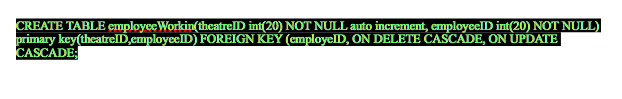
\includegraphics[scale=0.3]{sqlstatementempw.png}
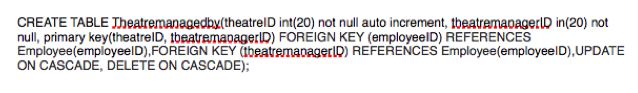
\includegraphics[scale=0.3]{theaterM.png}
\item{The Data Range Constraints used in the statement: }
Please insert the Data Range Constraints as follows:
\begin{itemize} 
	\item{The Data Access/update Constraint: }
	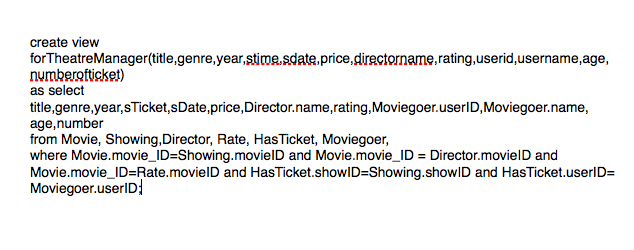
\includegraphics[scale=0.3]{forTheaterManager.png}
	\item{The Data Access/update Constraint Explanation:}
	For the theater manager view , the theater manager has access to everything in the database except the employees , because the chain manager takes care of that .The theatre manager can look up  cannot look at other users ID or passwords, name of employees or what type is each employee 
therefore, we create a view solely for the theater manager , so they can have access to the movie, showings, moviegoer entities so the theater manager can make any changes they want to movies in the system, showings and can make changes to the users in the system
	\item{The Data Access/update Constraint Example(s) (in correlation with the user(s) interaction with the system): } 
	When a theater manager wants to erase a showtime of a movie , it has access to do that , and other people cant
\end{itemize}
\item{The SQL statement to create the table: }
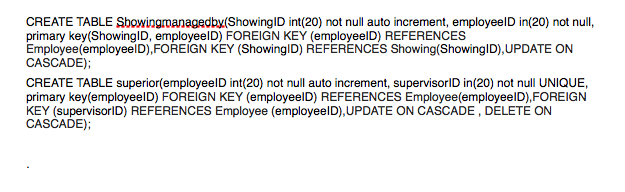
\includegraphics[scale=0.3]{last2tables.png}
\end{itemize}
Repeat that pattern for every table created.
}
